%contient des exemples d'homographies traité par nous et ripmap

\sse{Comparison of the Ripmap the new geometric-based decomposition}
%\sse{Comparaison du Ripmap et de la décomposition géométrique}

This part briefly describes the experiments shown in figures \ref{Homo1}, \ref{Homo2}, \ref{Homo3}, \ref{Homo4}, \ref{Homo5} and \ref{Homo5det}. Homographies far from degenerate ones have been chosen.

%Cette section décrit succintement les expériences représentées aux figures \ref{Homo1}, \ref{Homo2}, \ref{Homo3}, \ref{Homo4}, \ref{Homo5} et \ref{Homo5det}. On a choisit des homographies éloignées des cas dégénérés.


One can notice that the decompostion reduces aliasing on some homographies (homographies 1, 4 and 5). For a diagonal transforms it reduces the blur (homographie 2).Nevertheless for some homographies both the new method and the Ripmap give similar results (homographie 2). 


%On peut remarquer que la décomposition permet pour certaines homographies de limiter l'\emph{aliasing} (Homographies 1, 4 et 5). Dans le cas d'une déformation en diagonale elle limite le flou (Homographie 2). Il existe néanmoins des cas où les deux méthodes ont des performances comparables (Homographie 3).

The execution time of the program is about one second for an image of size $512\times 512$ on a dual-core laptop computer.

%Le programme a un temps d'éxecution de l'ordre d'une seconde sur une image $512\times 512$ avec un laptop à deux processeurs.

\begin{figure}
\subfigure[Geometric-based decomposition]{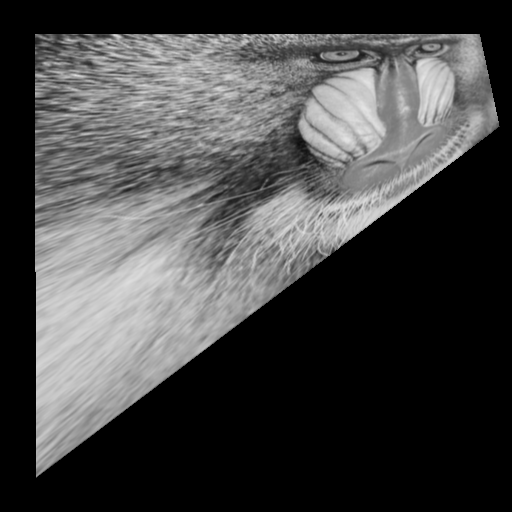
\includegraphics[scale=0.4]{img_f_1.png}}
\subfigure[Ripmap]{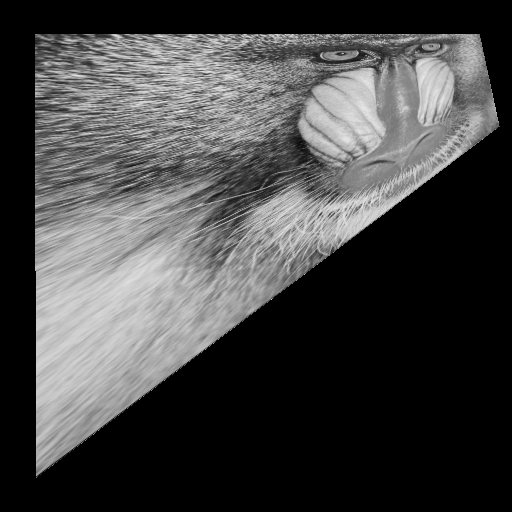
\includegraphics[scale=0.4]{img_ripmap_1.png}}
\caption{Homography 1 : The geometric-based decompostion method creates less aliasing}
\label{Homo1}
\end{figure}

%\begin{figure}
%\subfigure[Décomposition géométrique]{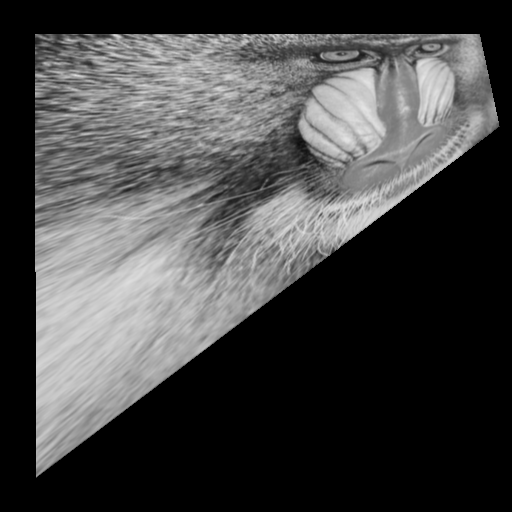
\includegraphics[scale=0.4]{img_f_1.png}}
%\subfigure[Ripmap]{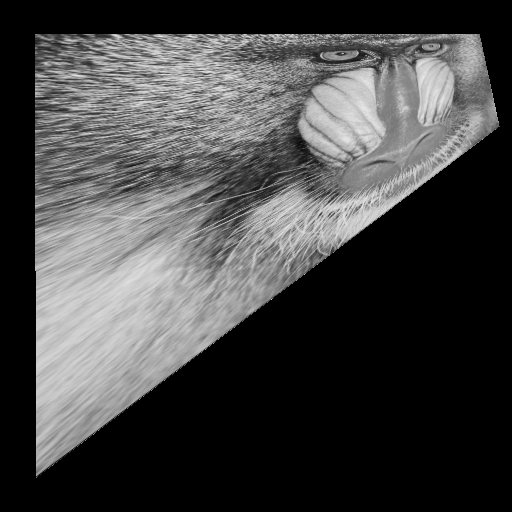
\includegraphics[scale=0.4]{img_ripmap_1.png}}
%\caption{Homographie 1 : La décomposition géométrique produit moins d'\emph{aliasing}}
%\label{Homo1}
%\end{figure}

\begin{figure}
\subfigure[Geometric-based decomposition]{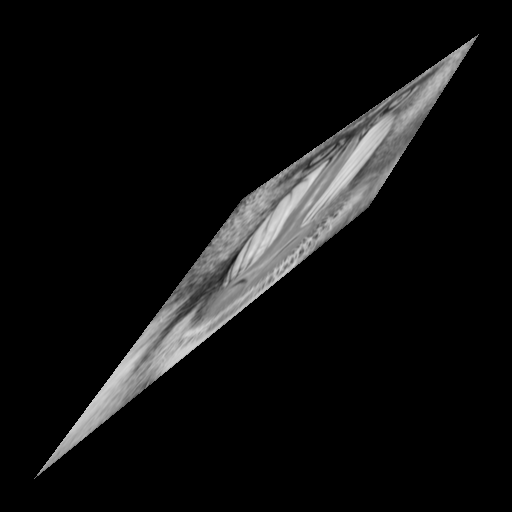
\includegraphics[scale=0.4]{img_f_2.png}}
\subfigure[Ripmap]{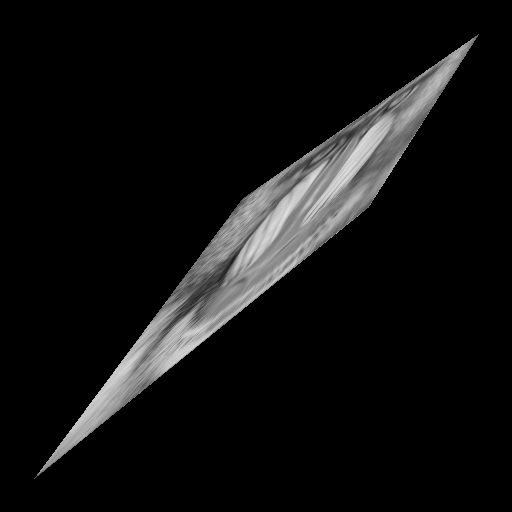
\includegraphics[scale=0.4]{img_ripmap_2.png}}
\caption{Homography 2 : The geometric-based decompostion method does not over-blur (see part \ref{Ripmap})}
\label{Homo2}
\end{figure}



%\begin{figure}
%\subfigure[Décomposition géométrique]{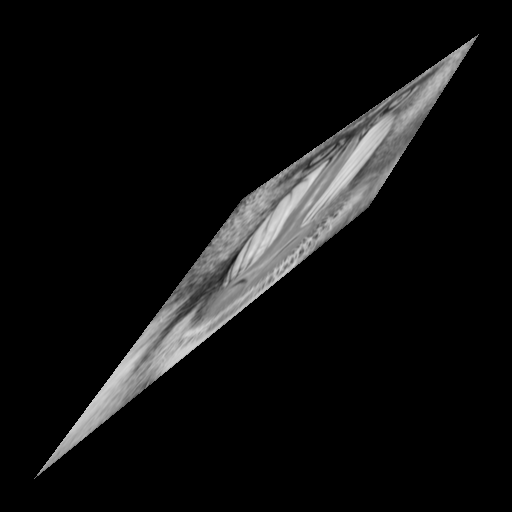
\includegraphics[scale=0.4]{img_f_2.png}}
%\subfigure[Ripmap]{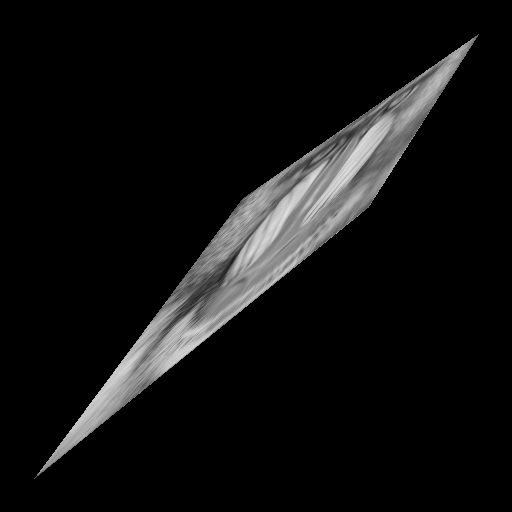
\includegraphics[scale=0.4]{img_ripmap_2.png}}
%\caption{Homographie 2 : La décomposition n'entraine pas d'\emph{over-blurring} (voir section \ref{Ripmap})}
%\label{Homo2}
%\end{figure}


\begin{figure}
\subfigure[Geometric-based decomposition]{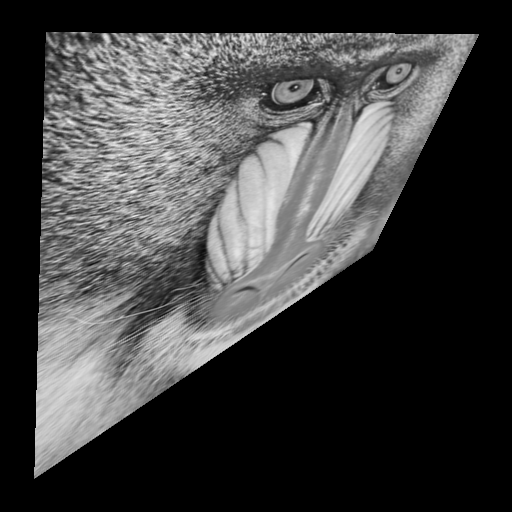
\includegraphics[scale=0.4]{img_f_3.png}}
\subfigure[Ripmap]{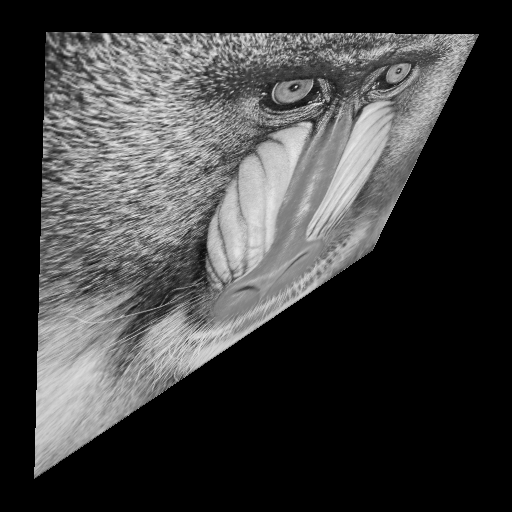
\includegraphics[scale=0.4]{img_ripmap_3.png}}
\caption{Homography 3 : None of the method seems to prevail}
\label{Homo3}
\end{figure}


%\begin{figure}
%\subfigure[Décomposition géométrique]{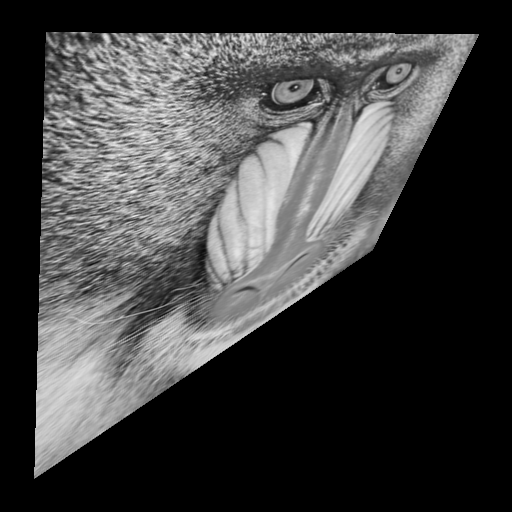
\includegraphics[scale=0.4]{img_f_3.png}}
%\subfigure[Ripmap]{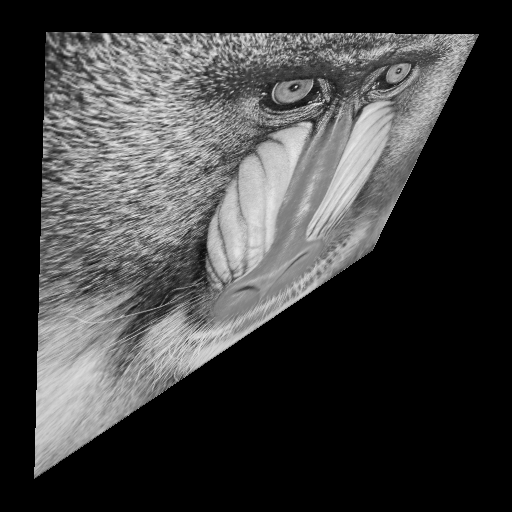
\includegraphics[scale=0.4]{img_ripmap_3.png}}
%\caption{Homographie 3 : Aucune des deux méthodes n'est clairement meilleure}
%\label{Homo3}
%\end{figure}

\begin{figure}
\subfigure[Geometric-based decomposition]{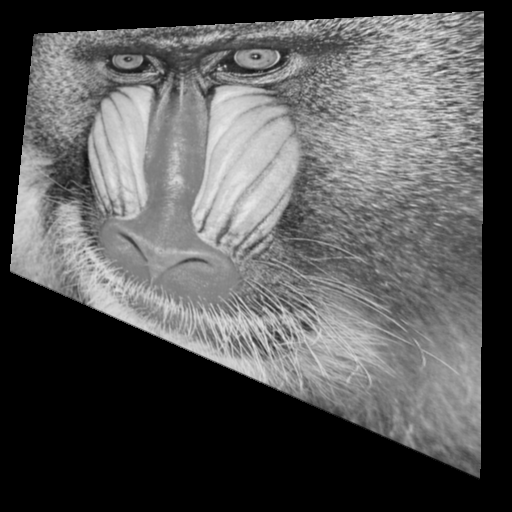
\includegraphics[scale=0.4]{img_f_4.png}}
\subfigure[Ripmap]{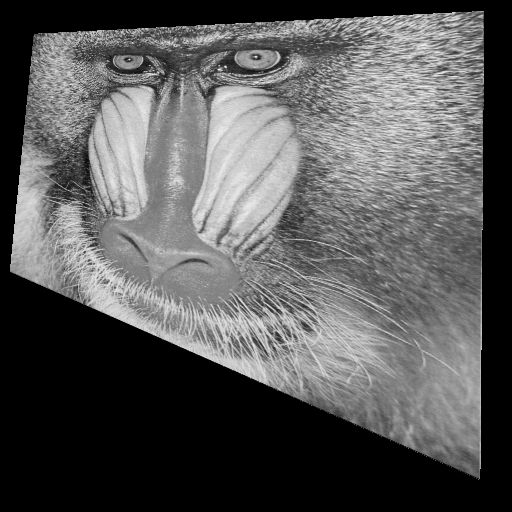
\includegraphics[scale=0.4]{img_ripmap_4.png}}
\caption{Homography 4 : The geometric-based decompostion method creates less aliasing}
\label{Homo4}
\end{figure}

%\begin{figure}
%\subfigure[Décomposition géométrique]{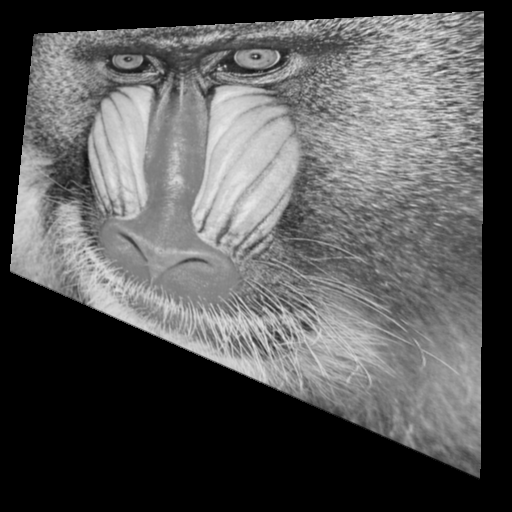
\includegraphics[scale=0.4]{img_f_4.png}}
%\subfigure[Ripmap]{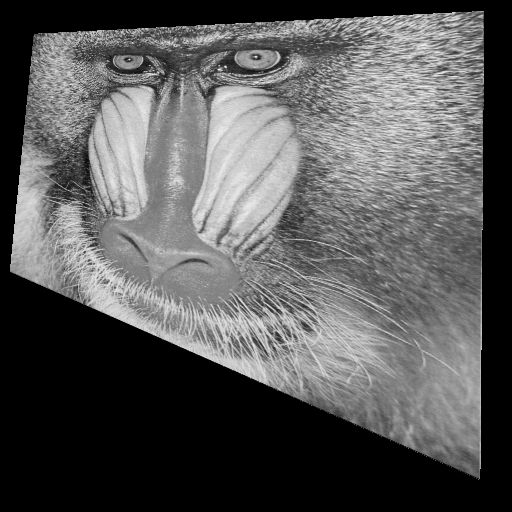
\includegraphics[scale=0.4]{img_ripmap_4.png}}
%\caption{Homographie 4 : La décomposition géométrique produit moins d'\emph{aliasing}}
%\label{Homo4}
%\end{figure}



\begin{figure}
\subfigure[Geometric-based decomposition]{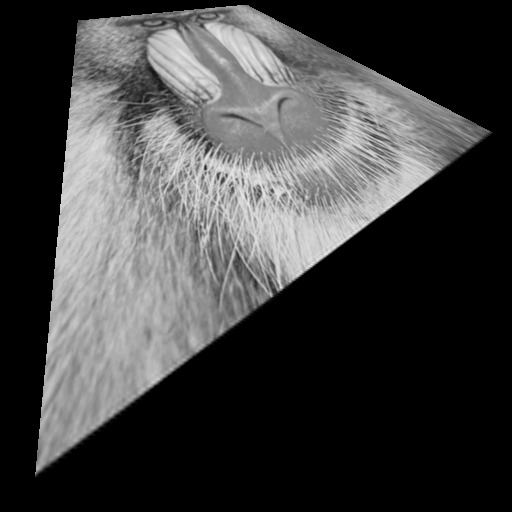
\includegraphics[scale=0.4]{img_geo_5.png}}
\subfigure[Ripmap]{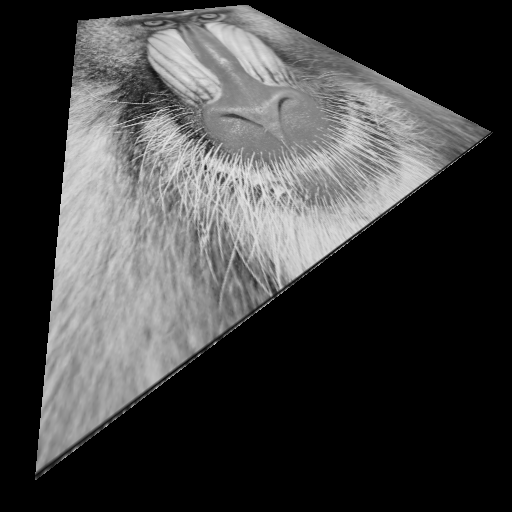
\includegraphics[scale=0.4]{img_ripmap_5.png}}
\subfigure[Naive method]{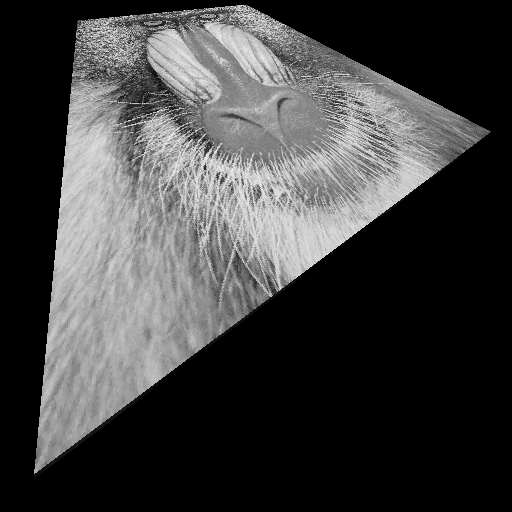
\includegraphics[scale=0.4]{img_naive_5.png}}
\subfigure[Mipmap]{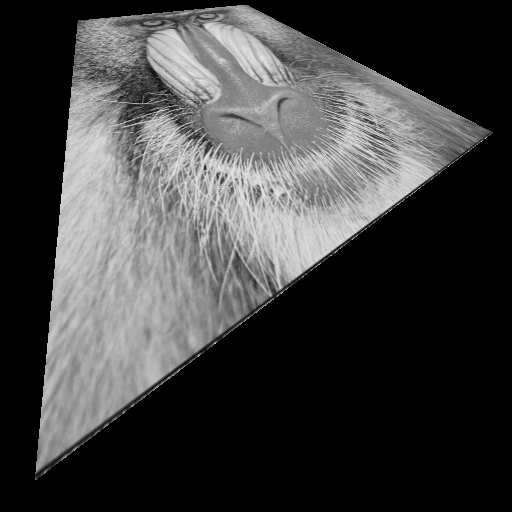
\includegraphics[scale=0.4]{img_mipmap_5.png}}
\caption{Homography 5 : The geometric-based decompostion method creates less aliasing. See the detail on figure \ref{Homo5det}}
\label{Homo5}
\end{figure}

%\begin{figure}
%\subfigure[Décomposition géométrique]{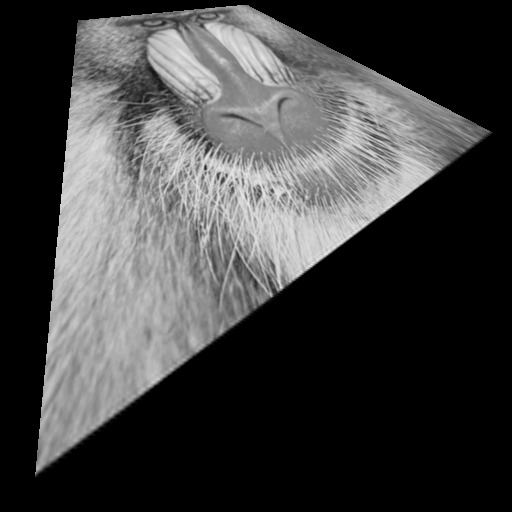
\includegraphics[scale=0.4]{img_geo_5.png}}
%\subfigure[Ripmap]{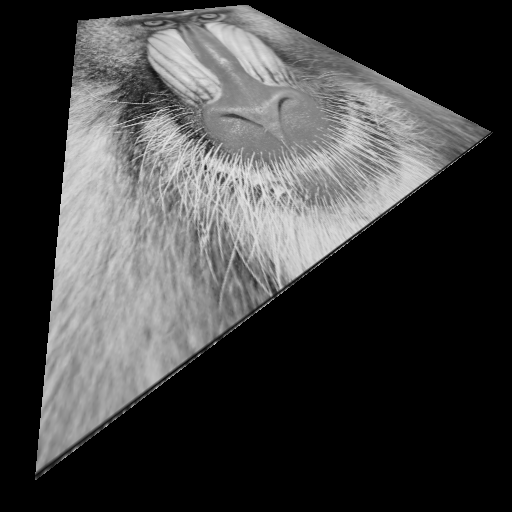
\includegraphics[scale=0.4]{img_ripmap_5.png}}
%\subfigure[Méthode naive]{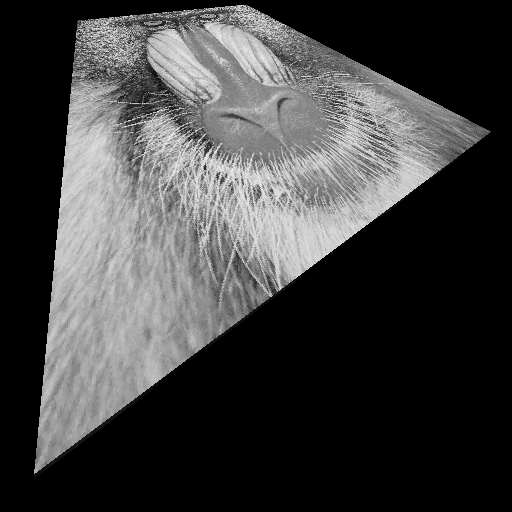
\includegraphics[scale=0.4]{img_naive_5.png}}
%\subfigure[Mipmap]{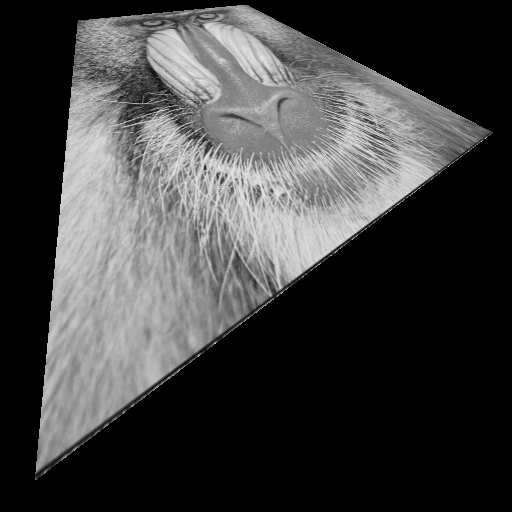
\includegraphics[scale=0.4]{img_mipmap_5.png}}
%\caption{Homographie 5 : La décomposition produit moins d'aliasing, un détail est présenté dans la figure \ref{Homo5det}}
%\label{Homo5}
%\end{figure}


\begin{figure}[t]
\centering
\subfigure[Naive method]{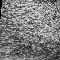
\includegraphics[scale=1.25]{img_det_naive.png}}\hfill
\subfigure[Mipmap]{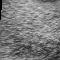
\includegraphics[scale=1.25]{img_det_mipmap.png}}\hfill
\subfigure[Ripmap]{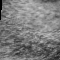
\includegraphics[scale=1.25]{img_det_ripmap.png}}\hfill
\subfigure[Geometric-based decomposition]{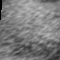
\includegraphics[scale=1.25]{img_det_geo.png}}
\caption{Detail of homographie 5 from figure \ref{Homo5} }
\label{Homo5det}
\end{figure}



%\begin{figure}[t]
%\centering
%\subfigure[Méthode naive]{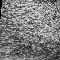
\includegraphics[scale=1.25]{img_det_naive.png}}\hfill
%\subfigure[Mipmap]{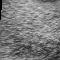
\includegraphics[scale=1.25]{img_det_mipmap.png}}\hfill
%\subfigure[Ripmap]{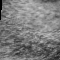
\includegraphics[scale=1.25]{img_det_ripmap.png}}\hfill
%\subfigure[Décomposition géométrique]{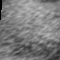
\includegraphics[scale=1.25]{img_det_geo.png}}
%\caption{Détail de l'homographie 5 qui a été présentée dans la figure \ref{Homo5} }
%\label{Homo5det}
%\end{figure}
